%% Compile: pdflatex > biber > pdflatex > pdflatex, or: latexmk -pdf researchproposal

\documentclass[11pt,a4paper]{article}

\usepackage[utf8]{inputenc}
\usepackage[T1]{fontenc}
\usepackage{textcomp}
\usepackage{lmodern}
\usepackage[british]{babel}

\usepackage[
  a4paper,
  top    = 2.5cm,
  bottom = 2.5cm,
  left   = 3.0cm,
  right  = 2.5cm,
]{geometry}

\usepackage{setspace}
\onehalfspacing
\setlength{\parindent}{0pt}
\setlength{\parskip}{6pt plus 2pt minus 1pt}

\usepackage{csquotes}
\usepackage[
  backend = biber,
  style   = apa,
  sorting = nyt,
  natbib  = true,
]{biblatex}
\DeclareLanguageMapping{british}{british-apa}
\addbibresource{bibliography.bib}

\usepackage{amsmath,amssymb}
\usepackage{bm}

\usepackage{tikz}
\usetikzlibrary{positioning, arrows, calc, shapes.geometric,
  fit, backgrounds}

\usepackage{booktabs}
\usepackage{longtable}
\usepackage{tabularx}
\usepackage{array}
\usepackage{multirow}
\usepackage{graphicx}
\usepackage{float}
\usepackage{xcolor}

\definecolor{thesisNavy}{HTML}{1F3A5F}
\definecolor{thesisTeal}{HTML}{2A7F8C}
\definecolor{thesisOrange}{HTML}{D97706}
\definecolor{thesisRed}{HTML}{C44536}
\definecolor{thesisGreen}{HTML}{4A7C59}
\definecolor{thesisGrey}{HTML}{6B7280}
\definecolor{thesisLight}{HTML}{F3F4F6}

\newcolumntype{L}[1]{>{\raggedright\arraybackslash}p{#1}}
\newcolumntype{C}[1]{>{\centering\arraybackslash}p{#1}}

\usepackage[font=small, labelfont=bf, skip=4pt]{caption}

\usepackage[
  colorlinks        = true,
  linkcolor         = blue!60!black,
  citecolor         = blue!60!black,
  urlcolor          = blue!60!black,
  pdftitle          = {Research Proposal -- Decomposition of Global Minimum Tax Revenue},
  pdfauthor         = {Maurits de Haan},
  pdfsubject        = {MSc Economic Policy Research Proposal -- Utrecht University},
  pdfkeywords       = {global minimum tax; Pillar Two; CbCR; revenue estimation; profit shifting},
  bookmarksopen     = true,
  bookmarksnumbered = true,
]{hyperref}

\usepackage{titlesec}
\titleformat{\section}{\large\bfseries}{\thesection}{1em}{}
\titleformat{\subsection}{\normalsize\bfseries}{\thesubsection}{1em}{}
\titleformat{\subsubsection}{\normalsize\itshape}{\thesubsubsection}{1em}{}

\usepackage{fancyhdr}
\pagestyle{fancy}
\fancyhf{}
\fancyhead[L]{\small\itshape Research proposal}
\fancyhead[R]{\small\itshape de Haan (\the\year)}
\fancyfoot[C]{\small\thepage}
\renewcommand{\headrulewidth}{0.4pt}
\renewcommand{\footrulewidth}{0pt}

\fancypagestyle{plain}{%
  \fancyhf{}
  \fancyfoot[C]{\small\thepage}
  \renewcommand{\headrulewidth}{0pt}
}

\newcommand{\GMT}{GMT}
\newcommand{\GloBE}{GloBE}
\newcommand{\ETR}{ETR}
\newcommand{\SBIE}{SBIE}
\newcommand{\CbCR}{CbCR}
\newcommand{\MNE}{MNE}
\newcommand{\EUR}{\texteuro}
\newcommand{\code}[1]{\texttt{#1}}

\begin{document}

\begin{titlepage}
  \thispagestyle{empty}
  \begin{center}

    \vspace*{1.5em}
    {\large\bfseries Utrecht University School of Economics}\\[0.3em]

    
\includegraphics[height=2.5cm]{UU_logo_2021_EN_RGB.png}\\[0.8em]

    \rule{\textwidth}{1pt}\\[1.2em]

    {\Large\bfseries
      Research Proposal\\[0.4em]
      Master Thesis U.S.E.}\\[1.0em]

    {\LARGE\bfseries
      Decomposition of Global Minimum Tax\\[0.3em]
      Revenue Using CbCR Data:
      \footnote{The copyright of this research proposal rests with the author. The author is responsible for its contents and opinions expressed. U.S.E.\ is only responsible for academic coaching and supervision and cannot be held liable for the content. I am grateful to dr.\ Peter Gerbrands for valuable comments and discussions.}}%
    \\[0.6em]
    {\large\itshape A factorial decomposition to quantifying uncertainty in\\[0.2em]
      EU revenue estimates under Pillar Two}\\[1.2em]

    \rule{\textwidth}{1pt}\\[2.0em]

    {\large Maurits de Haan}\\[0.3em]
    {\normalsize\href{mailto:m.c.p.dehaan@students.uu.nl}
      {m.c.p.dehaan@students.uu.nl}}\\
    {\normalsize\href{mailto:maurits.cpdehaan@gmail.com}
      {maurits.cpdehaan@gmail.com}}\\[2.0em]

    \begin{tabular}{@{}rl@{}}
      \textbf{Supervisor:} & dr.\ Peter Gerbrands \\[0.4em]
      \textbf{Second reader:} & dr.\ Adriaan Kalwij \\[0.4em]
      \textbf{Programme:} & MSc Economic Policy \\[0.4em]
      \textbf{University:} & Utrecht University \\[0.4em]
      \textbf{Academic year:} & 2025--2026 \\[0.4em]
      \textbf{Date:} & \today \\
    \end{tabular}

    \vfill

    \begin{tabular}{@{}ll@{}}
      \textbf{JEL codes:} &
        H25, H26, F23, H87 \\[0.5em]
      \textbf{Keywords:} &
        \parbox[t]{0.75\textwidth}{global minimum tax, Pillar Two,
        country-by-country reporting,\\
        revenue estimation, effective tax rate, profit shifting, BEPS}
    \end{tabular}

  \end{center}
\end{titlepage}

\newpage
\thispagestyle{plain}
\setcounter{page}{1}

\section{Introduction}\label{sec:introduction}

The Global Minimum Tax (GMT) is the most consequential reform of international corporate taxation since the post-war tax treaty network, and the revenue it raises for EU Member States remains poorly understood. Agreed in October 2021 by 137 jurisdictions under the OECD/G20 Inclusive Framework, the GMT imposes a minimum effective tax rate (ETR) of 15\% on the profits of multinational enterprises (MNEs) with consolidated revenues above \EUR750 million. It responds to four decades of profit shifting, the magnitude of which estimates place between roughly \$300 and \$850 billion annually \citep{torslov2023,garcia-bernardo2024,blouin2023,cobham2018}. By early 2026, more than sixty jurisdictions had enacted GMT legislation, yet no consensus exists on how much revenue the reform will raise, where it will accrue, or which design features drive the variation. This thesis estimates EU revenue, decomposes the uncertainty around that estimate, and separates the part driven by the data from the part driven by modelling choices.

Revenue estimates diverge. \citet{barake2022} compute a global gain of \EUR179 billion on the 2017 CbCR data, of which roughly \EUR55 billion would accrue to the EU. \citet{boukal2026} project a 4.3--5.3\% rise in Slovak corporate tax revenue, with roughly half from new top-up tax and half from reduced profit shifting. \citet{hugger2026}, drawing on OECD ETR percentile data at the UPE--affiliate level, show that 53.2\% of all low-taxed profit sits in jurisdictions whose \emph{average} ETR is at or above 15\%, so estimates that apply the jurisdiction-average ETR ignore more than half of the GMT base. There are no studies that decompose the GMT revenue within-jurisdiction and show the sources of divergence between jurisdictions. 

Three design features of the GMT compound the uncertainty. The top-up tax applies only to the fraction of profit taxed below the 15\% floor, so revenue depends on how within-jurisdiction ETR heterogeneity is measured \citep{hugger2026,bobeldijk2019}. The Substance-Based Income Exclusion (SBIE) shields a fraction of profit proportional to payroll and tangible assets, converting the headline 15\% rate into an effective floor that \citet{devereux2023} estimate at only 6.45\% in the first transition year for the average in-scope EU subsidiary. The tax semi-elasticity of reported profits is highly nonlinear: \citet{dowd2017} find a profit response six times larger at a 5\% statutory rate than at 30\%, well above the cross-study consensus semi-elasticity of 0.8 \citep{heckemeyer2017}. The January 2026 OECD Administrative Guidance added the Side-by-Side (SbS) Safe Harbour, under which MNE groups headquartered in jurisdictions with an eligible domestic and worldwide tax regime (in practice, only the United States) are removed from IIR and UTPR collection, and the Substance-Based Tax Incentive (SBTI) Safe Harbour, which permits qualifying tax incentives to be treated as additions to covered taxes up to a substance-based cap \citep{oecd2026}. No academic study quantifies their joint revenue consequences.

The thesis addresses the following research question:

\begin{quote}
\textit{What profit-shifting semi-elasticities emerge from the 2016--2022 CbCR panel under different functional forms, and how sensitive are the resulting Global Minimum Tax revenue estimates for EU Member States to the measurement of effective tax rates, the substance-based income exclusion, the implementation of the Side-by-Side package, and the specification of behavioural responses?}
\end{quote}

Three subquestions structure the analysis. SQ1 estimates the profit-shifting semi-elasticity on the 2016--2022 CbCR panel under linear, quadratic and logarithmic functional forms using the \citet{hines1994} framework with bilateral parent--affiliate fixed effects, and selects the preferred specification on the same sample. SQ2 embeds the preferred semi-elasticity alongside four further modelling choices in a $2^5$ full factorial design and decomposes the variance of the 32 resulting revenue scenarios through an ANOVA identity. SQ3 quantifies how the January 2026 Side-by-Side and SBTI Safe Harbours jointly reshape the magnitude and distribution of GMT revenue across EU Member States and across the QDMTT, IIR and UTPR collection channels.

The thesis expects four findings. The logarithmic specification dominates the linear and quadratic alternatives on the CbCR panel, and the panel semi-elasticity at $\tau = 0.05$ exceeds the meta-regression consensus of 0.8 \citep{heckemeyer2017} by at least a factor of three. In the factorial decomposition, ETR measurement accounts for the largest share of revenue variation, consistent with \citet{hugger2026}. Factor interactions exceed 10\% of total variance, so one-at-a-time sensitivity analysis understates the true uncertainty range. The SbS Safe Harbour turns net GMT revenue negative for Member States that rely on the UTPR channel and do not operate a Qualified Domestic Minimum Top-up Tax (QDMTT).

\subsection{Societal relevance}\label{sec:relevance}

The GMT is already being priced into European public budgets, and the projections rest on methodological choices whose sensitivity has not been academically tested. The Dutch Ministry of Finance has built \EUR466 million of projected GMT revenue into its medium-term fiscal framework, adjusted downward by \EUR122 million after the January 2026 Side-by-Side package \citep{36369_3,1028}. If the distributional ETR approach of \citet{hugger2026} roughly doubles the measured base, as their global figures imply, a single methodological switch moves the Dutch projection by hundreds of millions of euros. Therefore, it is needed that modelling choices to revenue are made explicit.

Additonally, tax competition puts pressure on government budgets \citep{cassee2019}, and the empirical evidence shows that low-income countries lose a disproportionate share of corporate tax revenue to profit shifting \citep{cobham2018,garcia-bernardo2024}. A replicable map of where GMT revenue will possibly land, and of how much of it will depend on assumptions, is needed for further negotiations during the implementation of the GMT. The thesis produces country-level estimates for all 27 EU Member States and attributes them to individual modelling choices, so that finance ministries, the European Commission and the OECD can read which assumption drove which number.

\subsection{Scientific contribution}\label{sec:contribution}

The thesis advances the GMT revenue literature on four fronts. First, it estimates the profit-shifting semi-elasticity on the 2016--2022 OECD CbCR panel with bilateral parent--affiliate fixed effects. Earlier studies only use data of one country \citep{dowd2017} or only one year \citep{garcia-bernardo2024}. The panel structure (2016-2022; pre-GMT implementation) used here allows for within-pair identification and bilateral fixed effects that absorb treaty networks, legal-system similarity and persistent features of MNE group structure. Linear, quadratic and logarithmic functional forms are compared on the same sample through. 

Second, the thesis embeds the panel-estimated semi-elasticity in a $2^5$ full factorial design over the five binary modelling choices: ETR measurement (jurisdiction-average vs.\ within-jurisdiction distributional), substance specification (aggregate vs.\ sectoral SBIE with an SBTI-capacity overlay), SBIE carve-out rates (initial vs.\ long-run), Side-by-Side regime (universal vs.\ SbS) and behavioural response (none vs.\ panel-estimated). The 32 resulting revenue surfaces are decomposed through an ANOVA identity that attributes the variation to main effects and interactions. \citet{barake2022} and \citet{hugger2026} vary parameters one at a time; \citet{boukal2026} decomposes by collection channel for a single country. The factorial design used here makes interactions simultaneously visible and decomposable across EU Member States. Policymakers can then read directly whether additional data or additional methodological clarity reduces uncertainty fastest.

Third, the thesis combines OECD CbCR aggregate levels with the post-2021 Eurostat Foreign Affiliates Statistics (FATS) sectoral shares to construct an effective tax floor matrix of 27 EU Member States. CbCR has no sectoral breakdown and FATS has no tax data; their combination fills a gap that \citet{devereux2023} and \citet{schjelderup2024} flag but do not resolve.

Fourth, the thesis cross-validates the percentile-based distributional ETR approach in CbCR Table I against the direct subsidiary-level observation in CbCR Table IV. No study has tested whether a five-percentile piecewise-uniform fit recovers the low-taxed profit share that Table IV observes directly. 

Section \ref{sec:litreview} reviews the empirical profit-shifting literature, the mechanics of the GMT base, and the theoretical modelling of tax competition under minimum taxation, and develops the five hypotheses that the thesis tests. Section \ref{sec:methodology} sets out the data, the panel specification and the factorial decomposition. Section \ref{sec:feasibility} discusses feasibility, risks and fall-back strategies. Section \ref{sec:timeline} lists the activities and milestones for period 4.

\newpage 

\section{Literature review and theoretical framework}\label{sec:litreview}

Three strands of literature inform the estimation framework: the empirical measurement of profit shifting, the mechanics of the GMT base, and the theoretical modelling of tax competition under minimum taxation.

\subsection{The empirical measurement of profit shifting}

Modern empirical work on profit shifting traces back to \citet{hines1994}, who regress the logarithm of reported profits on the tax rate while controlling for real economic activity through labour and capital inputs. The framework has yielded a meta-regression consensus semi-elasticity of approximately 0.8 \citep{heckemeyer2017,dharmapala2014,riedel2018}, with transfer pricing and intellectual property location accounting for 67--82\% of observed shifting and debt shifting responsible for the remainder. The meta-regression imposes a constant semi-elasticity across the ETR distribution, which masks nonlinearity that subsequent work has revealed but does not motivate how the semi-elasticity should behave at the very low rates the GMT targets.

Two studies establish that the constant-elasticity assumption breaks down exactly where the GMT bites. \citet{dowd2017} estimate a quadratic specification on US IRS Controlled Foreign Corporation returns for 2002--2012 and find semi-elasticities of 4.7 at a 5\% statutory rate and 0.7 at 30\%. In their simulation, raising six haven jurisdictions to a 29\% statutory rate removes \$116 billion of shifted profits under the quadratic model but only \$55--76 billion under a linear model. \citet{garcia-bernardo2024} replicate the pattern on a 2017 OECD CbCR cross-section with a logarithmic specification that permits unbounded semi-elasticity as $\tau \to 0$, and find total shifted profits of over \$850 billion. Neither study exploits within-pair time variation: Dowd is limited to US parents, and Garcia-Bernardo works on a single year. Both leave open the question whether the nonlinearity is a robust feature of the data or an artefact of bilateral heterogeneity that a pair fixed-effect estimator would absorb. The thesis takes exactly this step.

The macro-level literature supplies complementary magnitudes and a useful critique. \citet{torslov2023} use FATS to compare foreign- and locally-owned firm profitability and estimate that about 40\% of multinational foreign profits (\$616 billion in 2015) are shifted to tax havens; their approach is powerful at the aggregate level but attributes all excess profitability of foreign affiliates in tax havens to shifting, with no separation of real substance. \citet{garcia-bernardo2021} show, on an early CbCR vintage, that lower affiliate ETRs are associated with higher reported profits relative to every indicator of real economic activity, though their 2017 cross-section lacks the time dimension needed to absorb pair-specific confounders. \citet{cobham2018} re-estimate the spillover regressions of Crivelli, De Mooij and Keen and report global revenue losses of roughly \$500 billion annually, heavily concentrated in low-income countries, but the identifying variation is country-level and the mechanism is treated as a residual. \citet{blouin2023} challenge these magnitudes by demonstrating that standard data sources double-count foreign affiliate income through intermediate holding companies; their corrected measure reduces the \citet{clausing2016} US revenue loss from \$77--111 billion to roughly \$11 billion. The thesis takes this critique seriously through a holding-company-intensity correction that scales with the prevalence of intermediate holding companies in each affiliate jurisdiction, following the logic of \citet{garcia-bernardo2022a}.

The suitability of CbCR data itself has been questioned on methodological grounds. \citet{bobeldijk2019} argue that both the profit and the tax numerator in CbCR are structurally flawed as a basis for ETR-based risk assessment because of the treatment of intra-group dividends and the mismatch between accrued and paid taxes. \citet{godar2024}, working on voluntarily published firm-level CbCRs, show that inclusion of intra-company dividends is on average a minor concern but can be substantial for individual MNEs. The thesis addresses the critique by using the OECD's \code{PROFIT\_ADJ} measure where available and a predicted correction otherwise.

\subsection{The GMT base and the substance exclusion}

\citet{barake2022} produce the first systematic GMT revenue estimate by combining jurisdiction-average ETRs from CbCR with FATS-based corrections for double counting. They compute roughly \EUR179 billion globally and \EUR55 billion for the EU on the 2017 vintage, holding MNE behaviour fixed and assuming that all profit inside a jurisdiction faces that jurisdiction's average ETR. The jurisdiction-average assumption is the main limitation: it discards within-jurisdiction ETR heterogeneity.\footnote{\citet{barake2022} use the average because Table I alone contains no distributional information beyond the bilateral cell; the ETR percentiles that would permit a distributional approach were not yet released at the time of their study.} \citet{hugger2026} resolve this by exploiting the newly released OECD bilateral ETR percentile data (fifth, twenty-fifth, fiftieth, seventy-fifth and ninety-fifth percentiles at the UPE--affiliate level), and show that 53.2\% of all low-taxed profit sits in jurisdictions whose average ETR is at or above 15\%, so an approach that applies the jurisdiction-average ETR misses more than half of the global GMT base. Hugger fits a piecewise-uniform distribution between the five percentiles and a point mass below the fifth percentile. The thesis adopts this fit and extends it in two directions: the lower tail is spread as a uniform component on $[0, \tau^{(5)}]$ rather than collapsed to a point mass, so that near-zero-ETR profit is mathematically admissible; and the fit is cross-validated against the direct subsidiary-level \code{RATE\_0-15} observation in CbCR Table IV, which \citet{hugger2026} do not use.

\citet{devereux2023} provide the first empirical assessment of the Substance-Based Income Exclusion on Amadeus data for foreign-owned EU subsidiaries. The average SBIE-to-profit ratio is 57\% under initial carve-out rates and 41\% at long-run rates, so the average effective minimum tax on GloBE income is only 6.45\% in transition year one and 8.85\% in year ten. Around 30\% of in-scope EU subsidiaries have SBIE exceeding pre-tax profit and face zero top-up tax regardless of their ETR. The main limitation of the Devereux estimate is that Amadeus under-covers the largest MNEs (where the GMT actually bites) and over-represents smaller foreign-owned affiliates; the thesis therefore applies their conceptual framework to CbCR data that covers the relevant population by construction. \citet{devereux2022} show that the QDMTT rule order moves source countries to the head of the queue for the top-up tax, turning the GMT into a floor on tax collected by the source country rather than a uniform floor on total tax paid, and noting that the main competitive margin shifts to non-tax instruments such as subsidies. \citet{schjelderup2024} formalise the SBIE as a \emph{de facto} production subsidy that favours capital-intensive industries, with implicit capital subsidies of 0.50\% (buildings) to 0.96\% (machinery) dominating an implicit wage subsidy of at most 0.88\%. \citet{ferreiraliotti2022} add that the impact on existing tax incentives is highly uneven: accelerated depreciation is largely unaffected, while tax holidays and IP box regimes are mechanically neutralised by the top-up tax.

The thesis combines these insights into a two-stage substance filter: an aggregate SBIE-to-profit ratio, denoted $\phi$, computed directly from CbCR, and a sectoral version computed by applying FATS shares to CbCR aggregate levels.\footnote{The symbol $\phi$ is introduced in this thesis to denote the SBIE-to-profit ratio; \citet{devereux2023} compute the ratio without assigning it a symbol, \citet{schjelderup2024} work with absolute SBIE values. The ratio formulation makes the effective tax floor directly comparable across jurisdictions with different profit levels.} The sectoral version is then amplified by the January 2026 SBTI Safe Harbour, which permits qualifying tax incentives to be added to covered taxes up to a Substance Cap tied to payroll and tangible assets. The thesis derives a sector-level SBTI-capacity proxy $\kappa_{j,s}$ that measures how much room each sector has to protect local tax incentives without triggering the top-up tax, and includes it as an overlay in the substance filter.

\subsection{Theoretical models of tax competition under minimum taxation}

The welfare and competition consequences of the GMT have been modelled from several angles. \citet{johannesen2022} shows in a two-country model that the GMT is welfare-improving for non-haven countries when the profit-shifting semi-elasticity is large enough to offset the loss in firm-owner consumption; when the social welfare weight on private and public consumption is equalised, the threshold is a semi-elasticity of approximately 4. The meta-regression consensus of 0.8 falls far below this threshold, but the \citet{dowd2017} quadratic specification crosses the threshold at an ETR of about 9\%, which is precisely the range where the GMT bites. \citet{hebous2023} identify conditions under which a minimum tax combined with lump-sum transfers is Pareto-improving, but their framework is two-country and treats the SBIE stylistically. \citet{vantriet2025} simulate the GMT in CORTAX and find a welfare-optimal minimum rate of 16\%, with aggregate EU CIT revenue rising by about 6\%; the representative-firm framework cannot capture within-jurisdiction ETR heterogeneity or nonlinear semi-elasticities, and their main exercise assumes universal QDMTT implementation. \citet{janeba2023} show that the GMT removes the incentive for havens to undercut below 15\% but may intensify competition among non-havens through subsidies and regulatory concessions. \citet{jean2026} adds that enforcement cooperation may erode when a low-tax country's top-up is collected elsewhere.

\subsection{Conceptual framework}

The revenue pipeline treats the GMT as three multiplicative filters applied to the bilateral profit pool of each parent--affiliate pair: an ETR filter that isolates low-taxed mass, a substance filter that shields payroll and tangible assets, and a behavioural filter that removes the profit MNEs reallocate once the effective floor rises. The pre-allocation top-up liability is then distributed across QDMTT, IIR and UTPR collection channels under the January 2026 allocation rule. Five binary modelling choices enter the pipeline and generate the 32 scenarios individual and interactions analysed in the factorial decomposition. Figure \ref{fig:pipeline} summarises the set-up.

\begin{figure}[H]
\centering
\resizebox{\textwidth}{!}{%
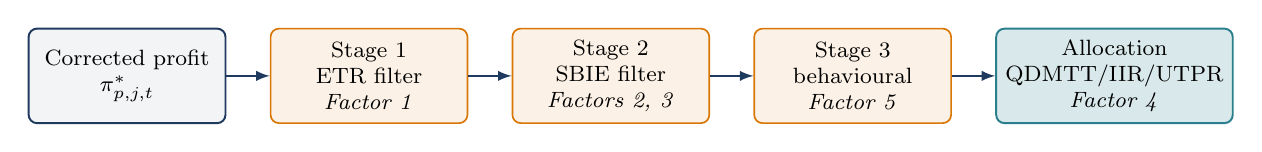
\begin{tikzpicture}[font=\small, node distance=0.75cm,
  stage/.style={draw=thesisNavy, line width=0.7pt, rounded corners=3pt,
                fill=thesisLight, minimum width=2.5cm, minimum height=1.2cm,
                align=center, font=\footnotesize},
  filt/.style={draw=thesisOrange, line width=0.6pt, rounded corners=3pt,
                fill=thesisOrange!10, minimum width=2.5cm, minimum height=1.2cm,
                align=center, font=\footnotesize},
  arr/.style={-latex, draw=thesisNavy, line width=0.7pt}]

  \node[stage] (input) {Corrected profit\\$\pi^{*}_{p,j,t}$};
  \node[filt, right=0.55cm of input] (s1) {Stage 1\\ETR filter\\\textit{Factor 1}};
  \node[filt, right=0.55cm of s1] (s2) {Stage 2\\SBIE filter\\\textit{Factors 2, 3}};
  \node[filt, right=0.55cm of s2] (s3) {Stage 3\\behavioural\\\textit{Factor 5}};
  \node[stage, right=0.55cm of s3, fill=thesisTeal!18, draw=thesisTeal]
        (alloc) {Allocation\\QDMTT/IIR/UTPR\\\textit{Factor 4}};

  \draw[arr] (input) -- (s1);
  \draw[arr] (s1) -- (s2);
  \draw[arr] (s2) -- (s3);
  \draw[arr] (s3) -- (alloc);
\end{tikzpicture}}
\caption[Three-stage revenue pipeline.]{The three-stage revenue pipeline. The allocation node routes the pre-allocation top-up liability through QDMTT, IIR or UTPR channels under the January 2026 Side-by-Side rule.}
\label{fig:pipeline}
\end{figure}

\subsection{Hypotheses}

\textbf{H1} The profit-shifting semi-elasticity is nonlinear across the ETR distribution and rises sharply at low ETRs. The logarithmic functional form captures this nonlinearity better than the linear or quadratic alternatives, and the panel estimate of the semi-elasticity at $\tau = 0.05$ exceeds the meta-regression consensus of 0.8 by a factor of at least three. The mechanism is that profit shifting via IP relocation and intra-group lending involves largely fixed set-up costs, so the marginal MNE finds shifting profitable at increasingly small tax differentials as $\tau \to 0$. \citet{bilicka2023} document exactly this pattern for IP ownership: 5\% of patents in the European market are sold in tax havens, and the response is concentrated in the largest MNEs.

\textbf{H2} The ETR measurement method accounts for the largest share of explained variance in the factorial decomposition. The mechanism follows from \citet{hugger2026}: switching from jurisdiction-average to within-jurisdiction distributional ETR measurement approximately doubles the measured GMT base. Subsequent filters act multiplicatively on that base, so the base effect dominates the variation unless behavioural responses or the SbS regime produce comparable shifts.

\textbf{H3} Factor interactions account for at least 10\% of total revenue variation. The mechanism is that the pipeline is multiplicative: the behavioural response removes a \emph{percentage} of the base, and whether that base was measured with the average or distributional approach alters the absolute effect. One-at-a-time sensitivity analysis cannot detect this interaction and understates the true uncertainty range.

\textbf{H4} The Side-by-Side Safe Harbour reduces aggregate EU GMT revenue collected through the IIR and UTPR channels, and the loss is concentrated in Member States that have not implemented a QDMTT. The SbS sets IIR and UTPR top-up to zero for MNE groups whose ultimate parent is in a jurisdiction with both an eligible domestic and an eligible worldwide tax regime (in practice, principally the United States), leaving the QDMTT as the only operative collection channel for that part of the base.

\textbf{H5} The SBTI Safe Harbour reduces the effective tax floor heterogeneously across EU sectors, and the reduction is largest in capital-intensive sectors. The mechanism follows from \citet{schjelderup2024}: the SBTI amplifies the SBIE's production-subsidy character, and capital-intensive sectors benefit doubly from the Substance Cap.

\section{Data and empirical strategy}\label{sec:methodology}

\subsection{Data}\label{sec:data}

Two primary datasets and several supplementary sources feed the estimation. The OECD Country-by-Country Reporting statistics \citep{oecd2025a} provide the bilateral parent--affiliate profit, tax, payroll, asset, and ETR-distribution data that form the backbone of the pipeline. The CbCR database is structured as six tables constructed from the same underlying filings but aggregated along different dimensions. Table I supplies jurisdiction-level financial aggregates together with five ETR percentiles $(P5, P25, P50, P75, P95)$ per bilateral cell, the only distributional shape information publicly available. Table IV partitions financial variables into 11 subsidiary-level ETR brackets, including the GMT-critical \code{RATE\_0-15} bracket, which directly observes low-taxed profit without any distributional extrapolation. The two tables complement each other: Table I has broader coverage (58 parent and 240 affiliate jurisdictions, 2016--2022) and supplies the percentile moments. Table IV has narrower coverage (49 parent and 154 affiliate jurisdictions) but observes the low-taxed profit mass directly. All 27 EU Member States appear in both tables. This allows the thesis to use Table IV as the preferred source on the EU sample and as the independent benchmark against which the Table I distributional fit is cross-validated.

CbCR data suffer from systematic double counting through intra-group dividends and intermediate holding companies \citep{blouin2023,garcia-bernardo2022a}. The OECD's \code{PROFIT\_ADJ} measure corrects this but first appears with broad coverage in 2021. The 2016--2020 panel is backcast using a jurisdiction-level prediction of the correction ratio as a function of holding-company intensity (from CbCR activity counts), regressed on the 2021--2022 observed ratio. 

Eurostat inward FATS provide the sectoral decomposition of economic activity that CbCR lacks, covering employment, turnover, personnel costs and investment. FATS supplies the sectoral \emph{shares} within each jurisdiction; CbCR supplies the aggregate \emph{levels}. Their combination yields the sector-specific SBIE estimates and the effective tax floor matrix of 27 EU Member States $\times$ 15--20 NACE sectors $\times$ 10 SBIE transition years.

Three supplementary datasets enter the estimation: statutory corporate income tax rates from the OECD Tax Database (as an instrument and robustness benchmark); OECD and ILO wage data (for imputing missing CbCR payroll values and as a control in the panel regressions); World Bank GDP per capita and population (as affiliate-jurisdiction controls). Pillar Two implementation status is tracked through the PwC global Pillar Two tracker, cross-referenced against the OECD Central Record of Qualified Domestic Minimum Taxes; this is the source of the QDMTT indicator and the SbS indicator used in the allocation stage.

\subsection{Methodology}\label{sec:estimation}

The key behavioural parameter of the revenue pipeline, the tax semi-elasticity of reported profits, is estimated directly from the 2016--2022 CbCR panel. The baseline specification follows \citet{hines1994}, adapted to a bilateral parent--affiliate panel:
\begin{equation*}
\log \pi_{p,j,t}^{*} = \beta_0 + \beta_1 \log A_{p,j,t} + \beta_2 \log \hat{W}_{p,j,t} + f(\tau_{p,j,t}) + \boldsymbol{\beta}_x \mathbf{X}_{p,j,t} + \alpha_{pj} + \gamma_t + \varepsilon_{p,j,t},
\end{equation*}
where $\pi^{*}$ is profit corrected for double counting, $A$ tangible assets, $\hat{W}$ payroll, $\tau$ the affiliate-level ETR, $\mathbf{X}$ log GDP per capita and log population of the affiliate jurisdiction, $\alpha_{pj}$ a parent--affiliate pair fixed effect and $\gamma_t$ a year fixed effect. The function $f(\tau)$ takes three forms, estimated on the same sample: $f_1(\tau) = \beta_3\,\tau$ (linear Hines--Rice), $f_2(\tau) = \beta_3\,\tau + \beta_4\,\tau^2$ (quadratic, \citealp{dowd2017}) and $f_3(\tau) = \beta_3\,\log(t+\tau)$ (logarithmic, \citealp{garcia-bernardo2024}, with $t$ a small offset that prevents the logarithm from diverging at zero).

The bilateral pair fixed effects absorb all time-invariant determinants of profit allocation: treaty networks, legal-system similarity, geographic proximity and persistent features of MNE group structure. Identification comes from within-pair variation in the ETR over 2016--2022, driven by domestic tax reforms (France 33.3\% $\to$ 25\%, Belgium 33.99\% $\to$ 25\%), the 2017 US Tax Cuts and Jobs Act, the compositional expansion of CbCR coverage and within-pair shifts in the mix of low-taxed and fully taxed profit. Year fixed effects absorb global shocks. \citet{garcia-bernardo2024} use the same Hines--Rice framework on a single cross-section, so their bilateral constants must be estimated through observable controls rather than absorbed by fixed effects; the panel here dispenses with that requirement.

The hypotheses in Section \ref{sec:litreview} map directly onto this specification. H1 predicts that the logarithmic form dominates the linear and quadratic alternatives and delivers a semi-elasticity at $\tau = 0.05$ that exceeds 0.8 by at least a factor of three. The BIC is the primary model selection criterion; the \citet{vuong1989} test formally compares the non-nested nonlinear alternatives; a non-parametric sample split by ETR quartile provides additional evidence on nonlinearity that does not rely on any specific functional form. The choice of functional form is decisive for the revenue estimates because the integrated top-up liability is concentrated in the lower tail of the ETR distribution, exactly where the three specifications disagree most.

Standard errors are clustered at the affiliate-jurisdiction level to allow for correlation across parents within the same affiliate. Two-way clustering (parent $\times$ affiliate) is reported as a robustness check, alongside the wild cluster bootstrap of \citet{cameron2008} for specifications in which the number of clusters is small. The preferred semi-elasticity is then embedded in the revenue pipeline, and the estimation uncertainty propagates through a pairs cluster bootstrap with 1,000 replications; each draw re-estimates the coefficients, recomputes counterfactual profits, and runs the full pipeline, producing a distribution of revenue estimates for every scenario--country cell.

Six robustness checks assess sensitivity: a balanced panel of pairs observed in all seven years; an instrumental-variable specification with lagged statutory CIT rates addressing the division bias in ETR measurement \citep{blouin2023}; a sample split by ETR quartile as non-parametric evidence for nonlinearity; a replication of the \citet{garcia-bernardo2024} specification on the 2017 slice to anchor the panel against the published cross-section; a sample excluding 2020--2021 to rule out COVID-driven variation; and winsorisation at the 1st and 99th ETR percentiles. If the within-pair standard deviation of the ETR has a median below two percentage points, a \citet{mundlak1978} correlated random-effects estimator is used as the fall-back, augmenting the specification with within-pair means of the time-varying regressors.

\subsection{Factorial decomposition}\label{sec:factorial}

The preferred semi-elasticity enters the revenue pipeline through a $2^5$ full factorial design. Each modelling choice is assigned one of two levels: Factor 1 switches ETR measurement between jurisdiction-average and within-jurisdiction distributional; Factor 2 switches substance specification between aggregate and sectoral SBIE with SBTI-capacity overlay; Factor 3 switches SBIE carve-out rates between initial (10\%/8\%) and long-run (5\%/5\%); Factor 4 switches the allocation rule between universal IIR/UTPR and the Side-by-Side Safe Harbour; Factor 5 switches the behavioural response between none and the panel-estimated nonlinear semi-elasticity.

Revenue is computed under all 32 configurations for each EU Member State and year. The ANOVA identity for a balanced $2^K$ design decomposes the total sum of squares exactly into 5 main effects, 10 two-way interactions, 10 three-way interactions, 5 four-way interactions and 1 five-way interaction, totalling the $2^5 - 1 = 31$ orthogonal contrasts that exhaust the total variation. The share attributable to each effect ($\eta_i^2 = SS_i / SS_{\text{total}}$) is reported at three levels: pooled across all EU Member States and years. 

The design separates two distinct sources of uncertainty. \emph{Scenario spread} is the range of revenue estimates across the 32 modelling configurations, driven by assumptions that cannot be resolved by more data. \emph{Estimation uncertainty} is the width of the bootstrapped confidence interval inside a single scenario, driven by the statistical precision of the semi-elasticity. The ratio of the two indicates whether reducing revenue uncertainty requires better data or better modelling; if the ratio exceeds one, modelling choices dominate and the priority for fiscal ministries is not more observations but more methodological clarity.

\section{Feasibility}\label{sec:feasibility}

The thesis is feasible on three counts: the data are in hand, the methods are standard, and the combination of the two has not been executed before. All raw data are already downloaded and catalogued. The originality lies in the combination and the addition of the latest Administrative Guidance. 

Three risks are acknowledged. First, within-pair ETR variation may be insufficient to identify the semi-elasticity; the Mundlak correlated random-effects specification is specified in advance as the fall-back, and the instrumental-variable alternative using lagged statutory rates is available if the Mundlak assumption itself is rejected. Second, the profit-base correction assumes structural stability in the holding-company--double-counting relationship over 2016--2022. This assumption is tested by estimating the correction model separately on 2021 and 2022 and comparing coefficients. Third, the CbCR data suffer from well-documented imperfections \citep{bobeldijk2019,godar2024,blouin2023}; the thesis mitigates these concerns in the entire calculation framework, and the scenario spread produced by the factorial design is precisely the object that quantifies the residual uncertainty.

\section{Activities and timeline}\label{sec:timeline}

Table \ref{tab:timeline} lists the planned activities from mid-April 2026 through the final deadline of 26 June 2026, with milestones marking the end of each block. Bi-weekly supervision meetings are scheduled throughout. The timeline works backward from the final thesis deadline, allocating roughly one third of the available weeks to data cleaning and panel estimation, one third to the factorial decomposition and robustness, and one third to writing, feedback collection and final revision. A one-week buffer is reserved in the final block.

\begin{table}[H]
\centering
\caption{Activities and timeline, period 4 (April--June 2026)}
\label{tab:timeline}
\small
\begin{tabular}{@{}L{3.2cm}L{5.8cm}L{4.8cm}@{}}
\toprule
\textbf{Dates} & \textbf{Activity} & \textbf{Milestone} \\
\midrule
14--27 Apr
  & Finalise research proposal; clean CbCR Table I and Table IV; compute jurisdiction-average and distributional ETRs; produce descriptive statistics of within-pair ETR variation.
  & Proposal submitted; cleaned CbCR panel and descriptive tables ready. \\[0.4em]
28 Apr--11 May
  & Implement profit-base correction (holding-company regression); merge FATS sectoral shares; construct effective tax floor matrix.
  & Stage 1 and Stage 2 inputs ready. \\[0.4em]
12--25 May
  & Estimate linear, quadratic and logarithmic semi-elasticities; run BIC, Vuong and robustness checks; draft semi-elasticity results section.
  & Panel estimation complete; SQ1/H1 addressed. \\[0.4em]
26 May--8 Jun
  & Run $2^5$ factorial design; ANOVA decomposition; pairs cluster bootstrap; country-level decompositions.
  & Factorial results and figures complete; SQ2/H2--H3 addressed. \\[0.4em]
9--15 Jun
  & SbS and SBTI analysis; draft results section for SQ3; draft discussion and policy implications.
  & SQ3/H4--H5 addressed; full draft ready. \\[0.4em]
15--23 Jun
  & Discuss draft with supervisor; incorporate feedback; finalise figures and tables; proofread in British English.
  & Revised draft ready for submission. \\[0.4em]
24--26 Jun
  & Final revisions; check references, abbreviations, figure numbering; submit.
  & Final thesis submitted (26 June). \\
\bottomrule
\end{tabular}
\end{table}

\newpage
\printbibliography[heading=bibintoc]

\end{document}
